\chapter{Aplikacja webowa do powiększania rozdzielczości obrazów}

Podczas korzystania z Internetu miałem kilka sytuacji w których potrzebowałem narzędzia, które pozwoli mi na powiększenie rozdzielczości obrazów. Stron internetowych tego typu jest wiele, sporo aplikacji do edycji zdjęć umożliwia powiększenie rozdzielczości obrazów, przykładem może być \textbf{Photoshop} i inne.

Korzystając z rozwiązań ogólnodostępnych zauważyłem, że darmowe aplikacje nie gwarantują wysokiej jakości obrazów wyjściowych, zaś bardziej rozbudowane rozwiązania są płatne lub mają dostępne tylko jedno powiększenie obrazu na dobę. 

Postanowiłem więc wykorzystac ogólnodostępne algorytmy rozwiązujące problem super-rozdzielczości, następnie użyć ich do aplikacji która w domyśle będzie darmowa i będzie dawała możliwość porównania wyników działania kilku algorytmów. Nie zawsze jedna z wdrożonych metod będzie dawać najlepsze wyniki, więc chciałbym żeby użytkownik miał wybór a pro po tego którą metodę chce wykorzystać.

Głównym założeniem aplikacji jest intuicyjność i minimalizacja interakcji potrzebnych do powiększenia obrazu; zauważyłem, że rozwiązania konkurencji wymagają akceptacji regulaminów, lub dopiero po przejściu kilku ekranów możemy wysłać obraz, którego rozdzielczość chcemy powiększyć. Uznałem to za bardzo ważne, gdyż użytkownicy chcą szybko dostać wynik, użytkownik nie będzie czekał nie wiadomo jak długo na wynik.

Nie spotkałem się z tym, żeby aplikacje innych firm pozwalały na porównanie wyników różnych algorytmów ze sobą. Uważam że to jest istotne gdy chcemy uzyskać wynik najwyższej jakości, bo jak wspomniałem nie ma rozwiązań idealnych i nie zawsze jedna z wdrożonych metod będzie dawać najlepsze wyniki.

Ważne jest dla mnie, żeby aplikacja była estetyczna i przyjemna dla oka. Dużo chętniej korzystamy z narzędzi czy urządzeń które lepiej wyglądają, bardziej się nam podobają i chciałbym żeby tak było w tym przypadku. W planie również jest dbanie o animacje i o to żeby interakcje z narzędziem były przyjemne i satysfakcjonujące.

\newpage
\begin{figure}[H]
    \begin{minipage}{\linewidth}
        \centering
        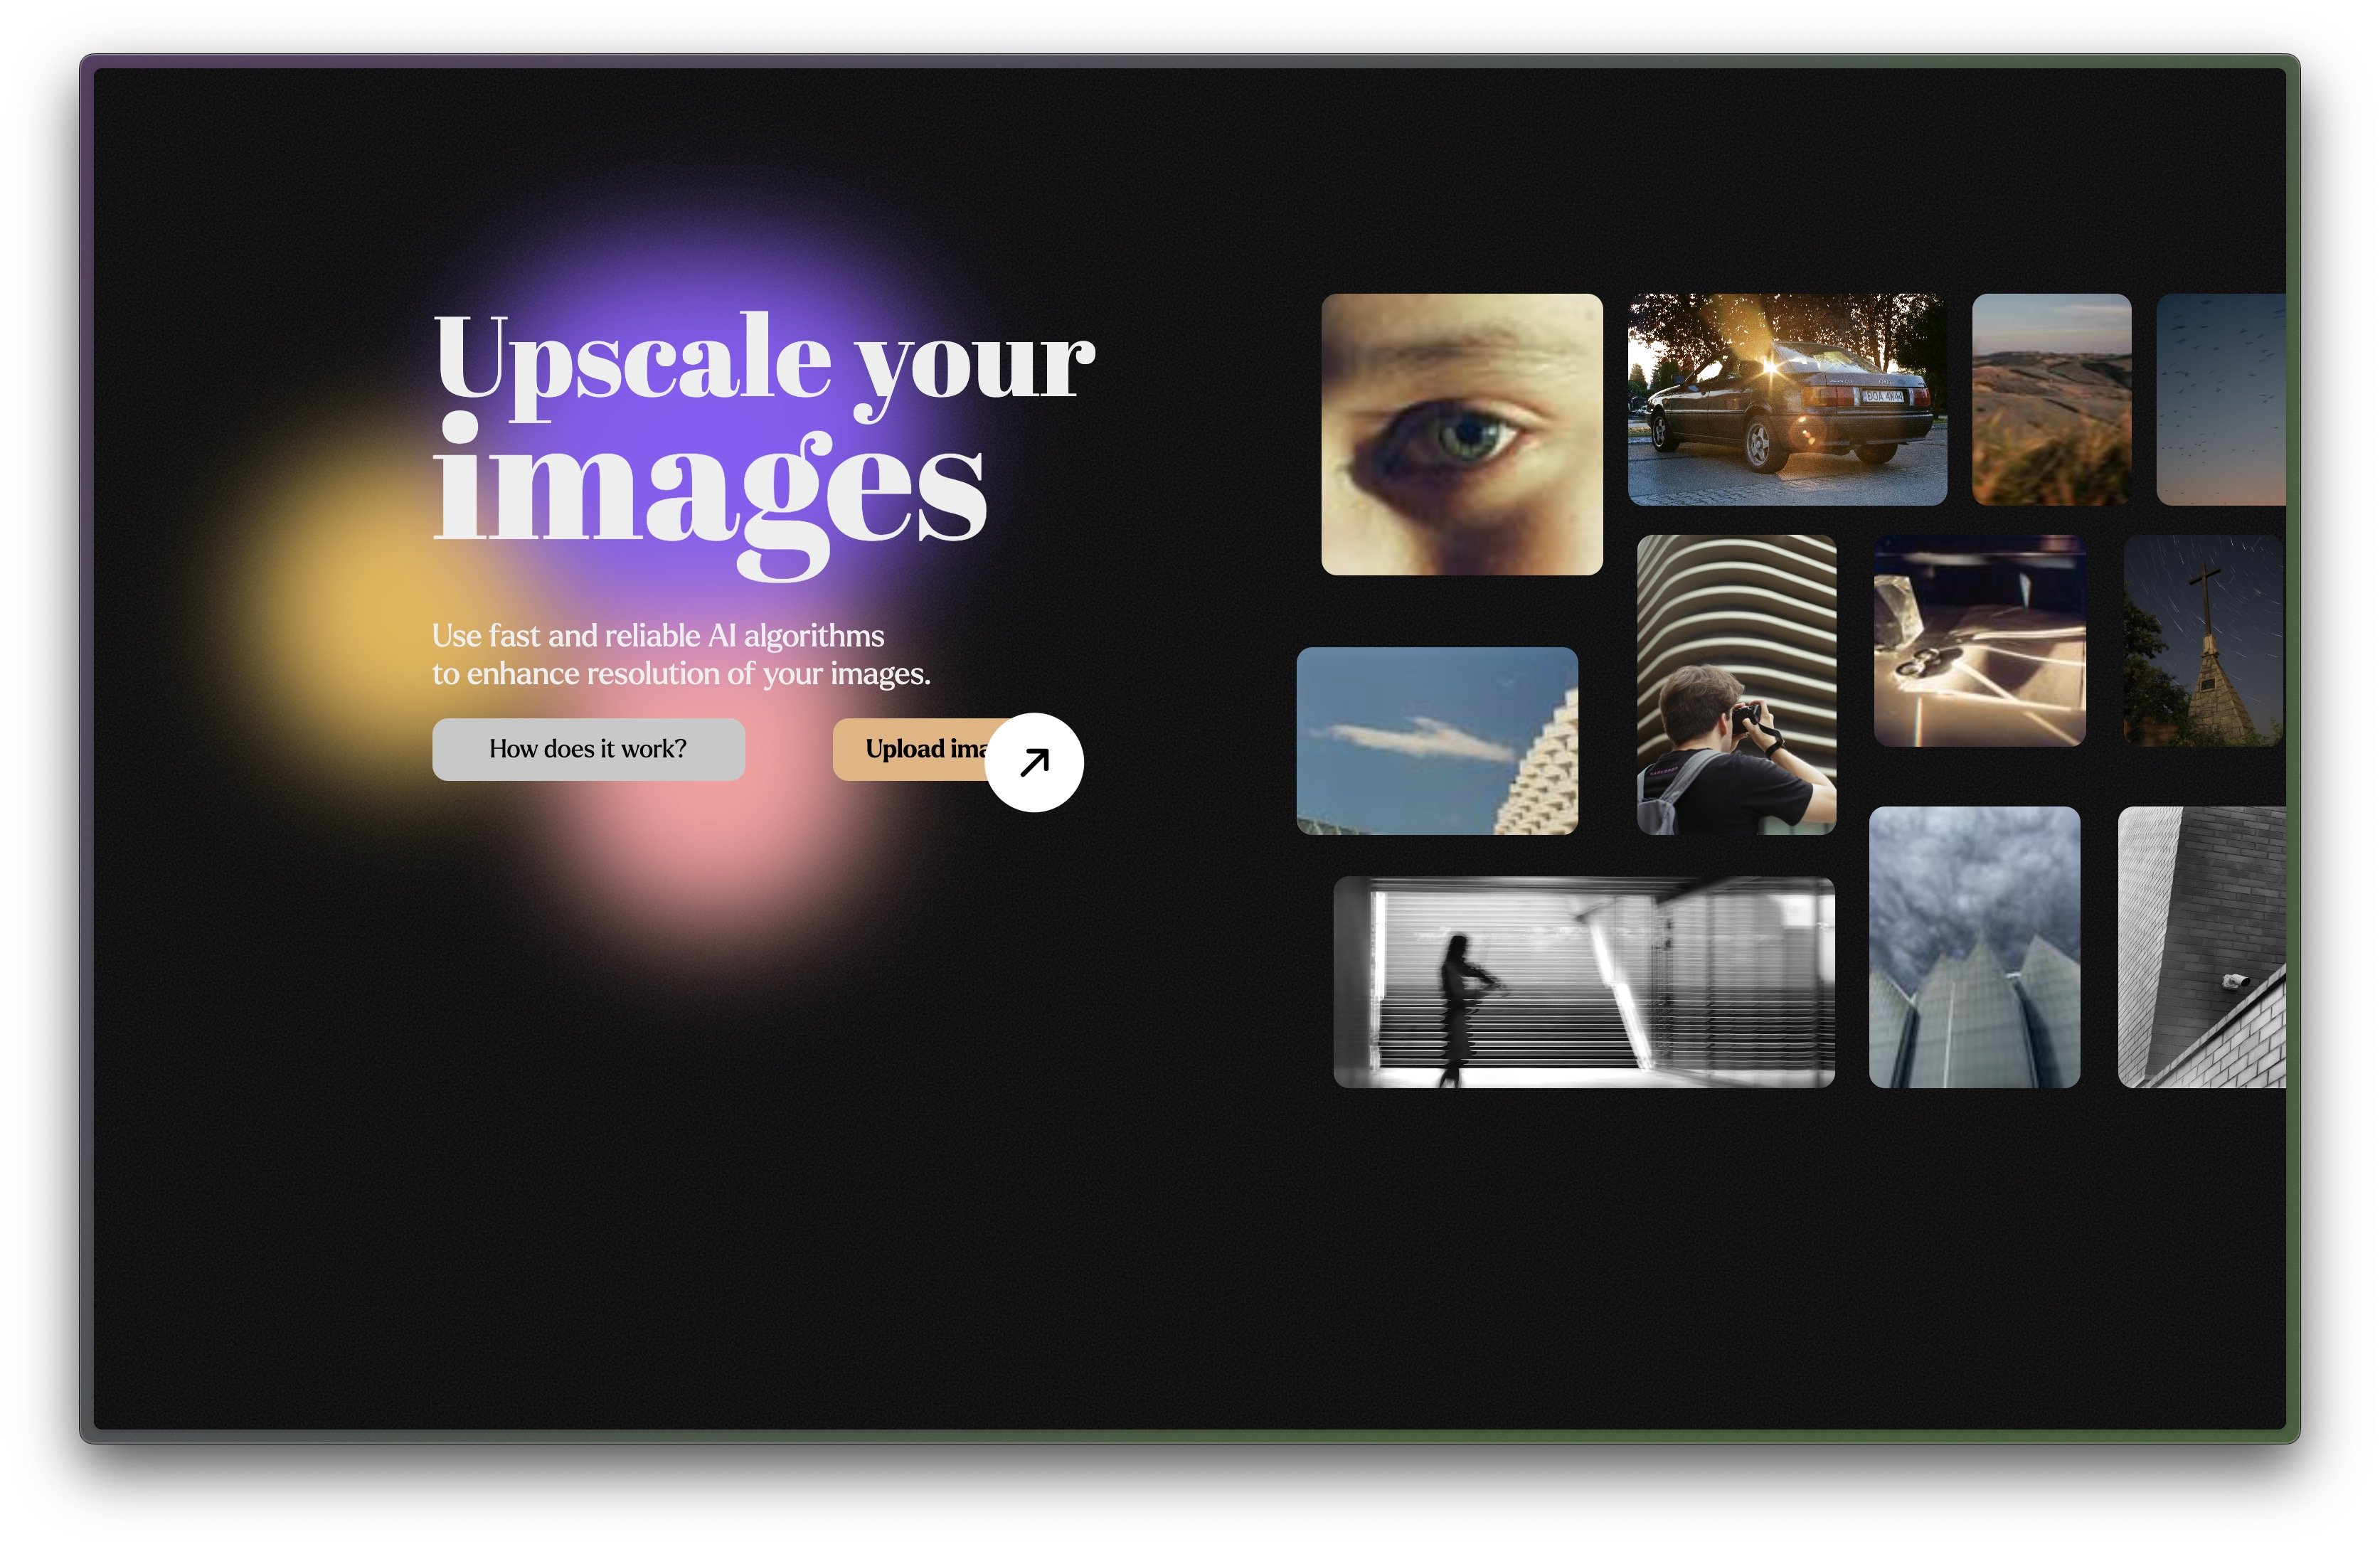
\includegraphics[width=0.8\linewidth]{Rozdziały/06.Aplikacja/Obrazy/kursor-link.png}  
        \caption{Widok strony głównej aplikacji}
        \label{fig:image80}
        \includegraphics[width=0.8\linewidth]{Rozdziały/06.Aplikacja/Obrazy/result-zoom.png}  
        \caption{Widok prezentacji wyników}
        \label{fig:image81}
    \end{minipage}
\end{figure}
\newpage

\section{Projektowanie aplikacji}

Pierwszym etapem tworzenia aplikacji było stworzenie diagramu przepływu użytkownika (user flow diagram) [Rys \ref{fig:image82}], który ilustruje kolejność interakcji użytkownika z aplikacją. Potencjalni użytkownicy mają już pewne oczekiwania i potrzeby, spodziewają się gdzie na ekranie znajdą się konkretne elementy. Dlatego ważne jest, żeby zrozumieć jak użytkownik będzie korzystał z aplikacji, jakie akcje będzie wykonywał i w jaki sposób będzie się poruszał po stronie.

\begin{figure}[ht]
    \centering
    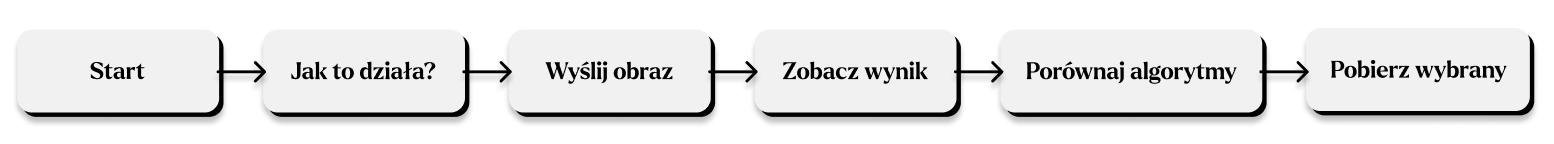
\includegraphics[width=\linewidth]{Rozdziały/06.Aplikacja/Obrazy/user-flow.png}  
    \caption{Diagram przepływu użytkownika}
    \label{fig:image82}
\end{figure}

Diagram ten przedstawia wszystkie interakcje, które użytkownik może wykonać w aplikacji. Te interakcje nie muszą być wykorzystane, ale są dostępne dla użytkownika.

Kolejnym krokiem był projekt interfejsu użytkownika. Zdecydowałem, że narzędzie będzie składać się z dwóch ekranów: ekranu głównego \ref{fig:image80}, oraz widoku prezentacji obrazu wynikowego \ref{fig:image81}.

Projekt wyglądu aplikacji rozpocząłem od rozrysowania wireframe'ów [Rys \ref{fig:image83}] z użyciem narzędzia \textbf{Figma}, służącym do projektów graficznych między innymi aplikacji. Wireframe'y to proste szkice, które pozwalają na zobrazowanie układu elementów na stronie. Elementy te odpowiadają za funkcjonalność, a nie wygląd aplikacji i są ściśle powiązane z diagramem przepływu użytkownika.

\begin{figure}[ht]
    \centering
    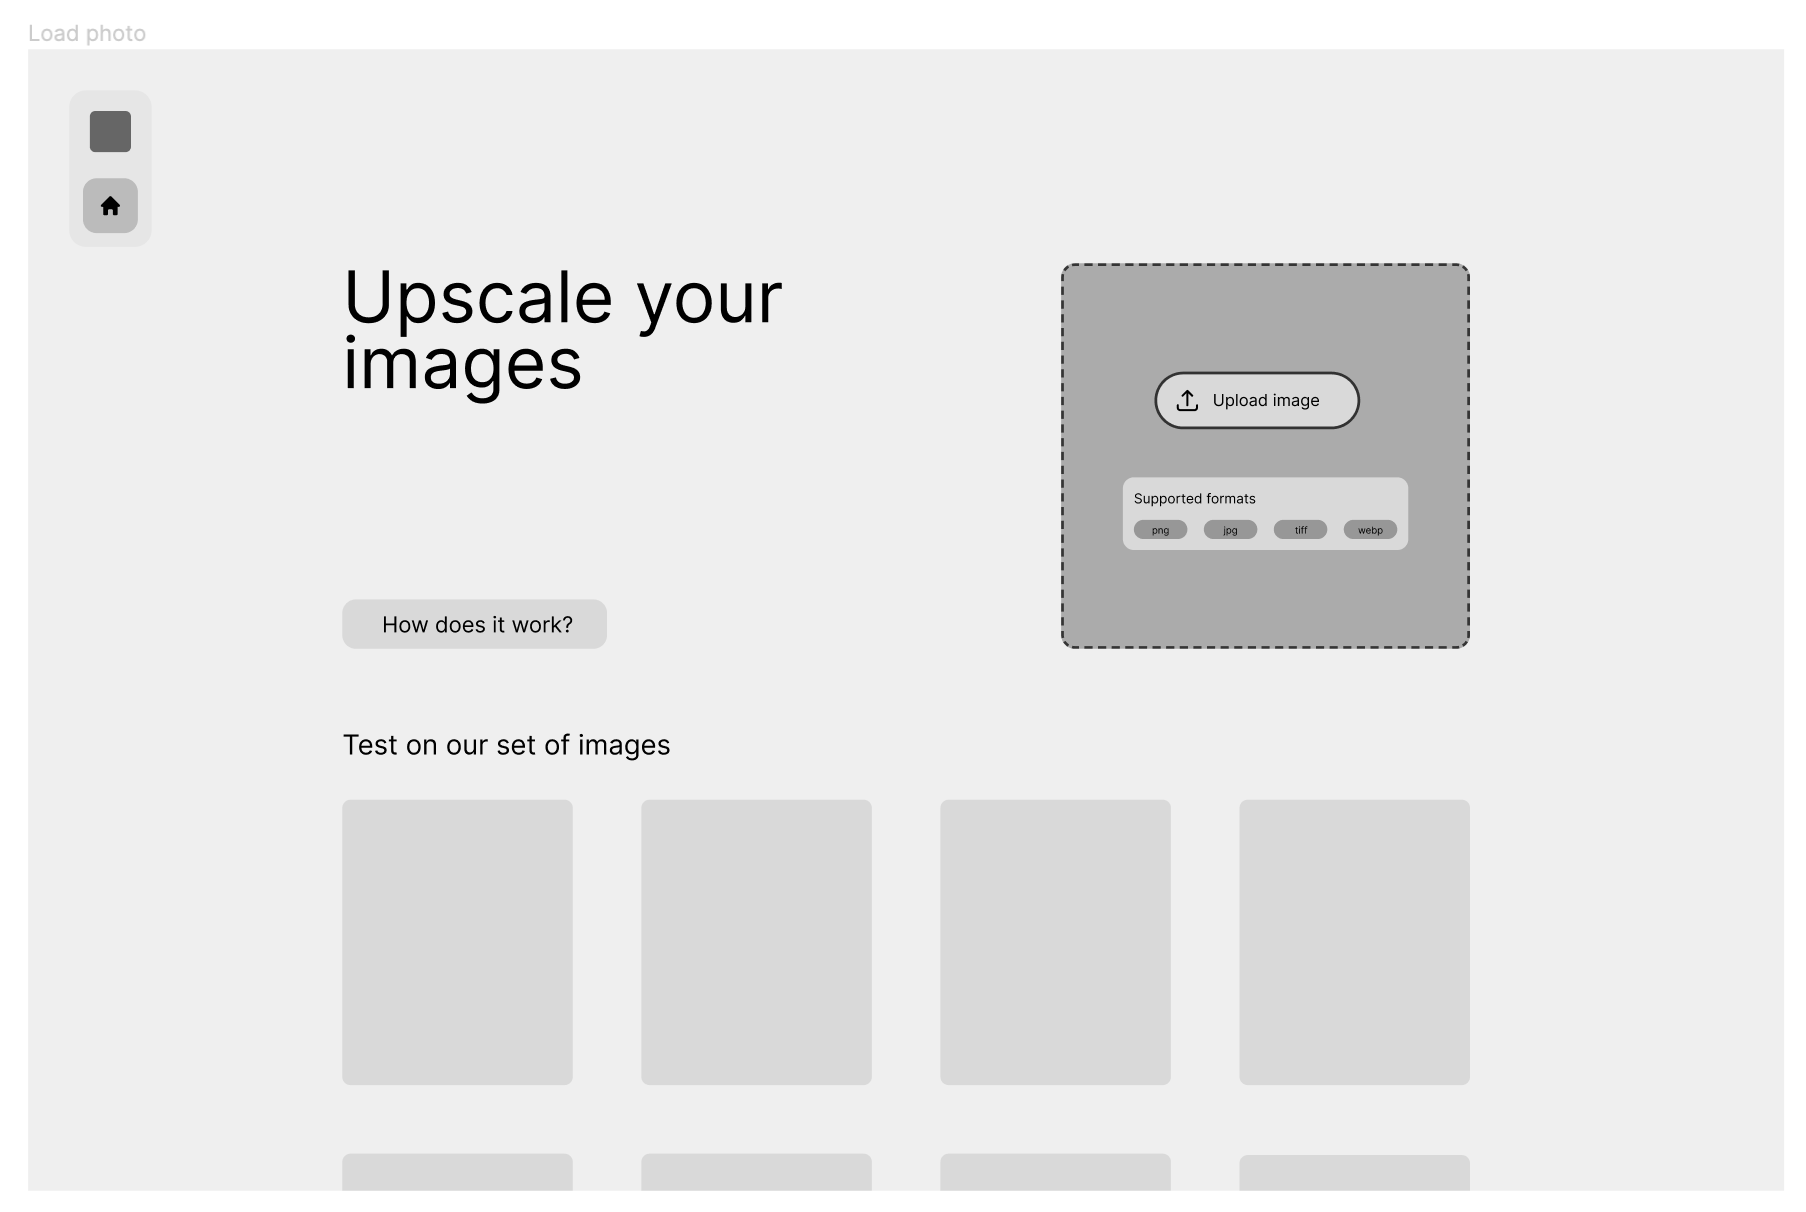
\includegraphics[width=0.8\linewidth]{Rozdziały/06.Aplikacja/Obrazy/UX upload.png}  
    \caption{Pierwsza wersja UX aplikacji (ekran główny)}
    \label{fig:image83}
\end{figure}

\begin{figure}[ht]
    \centering
    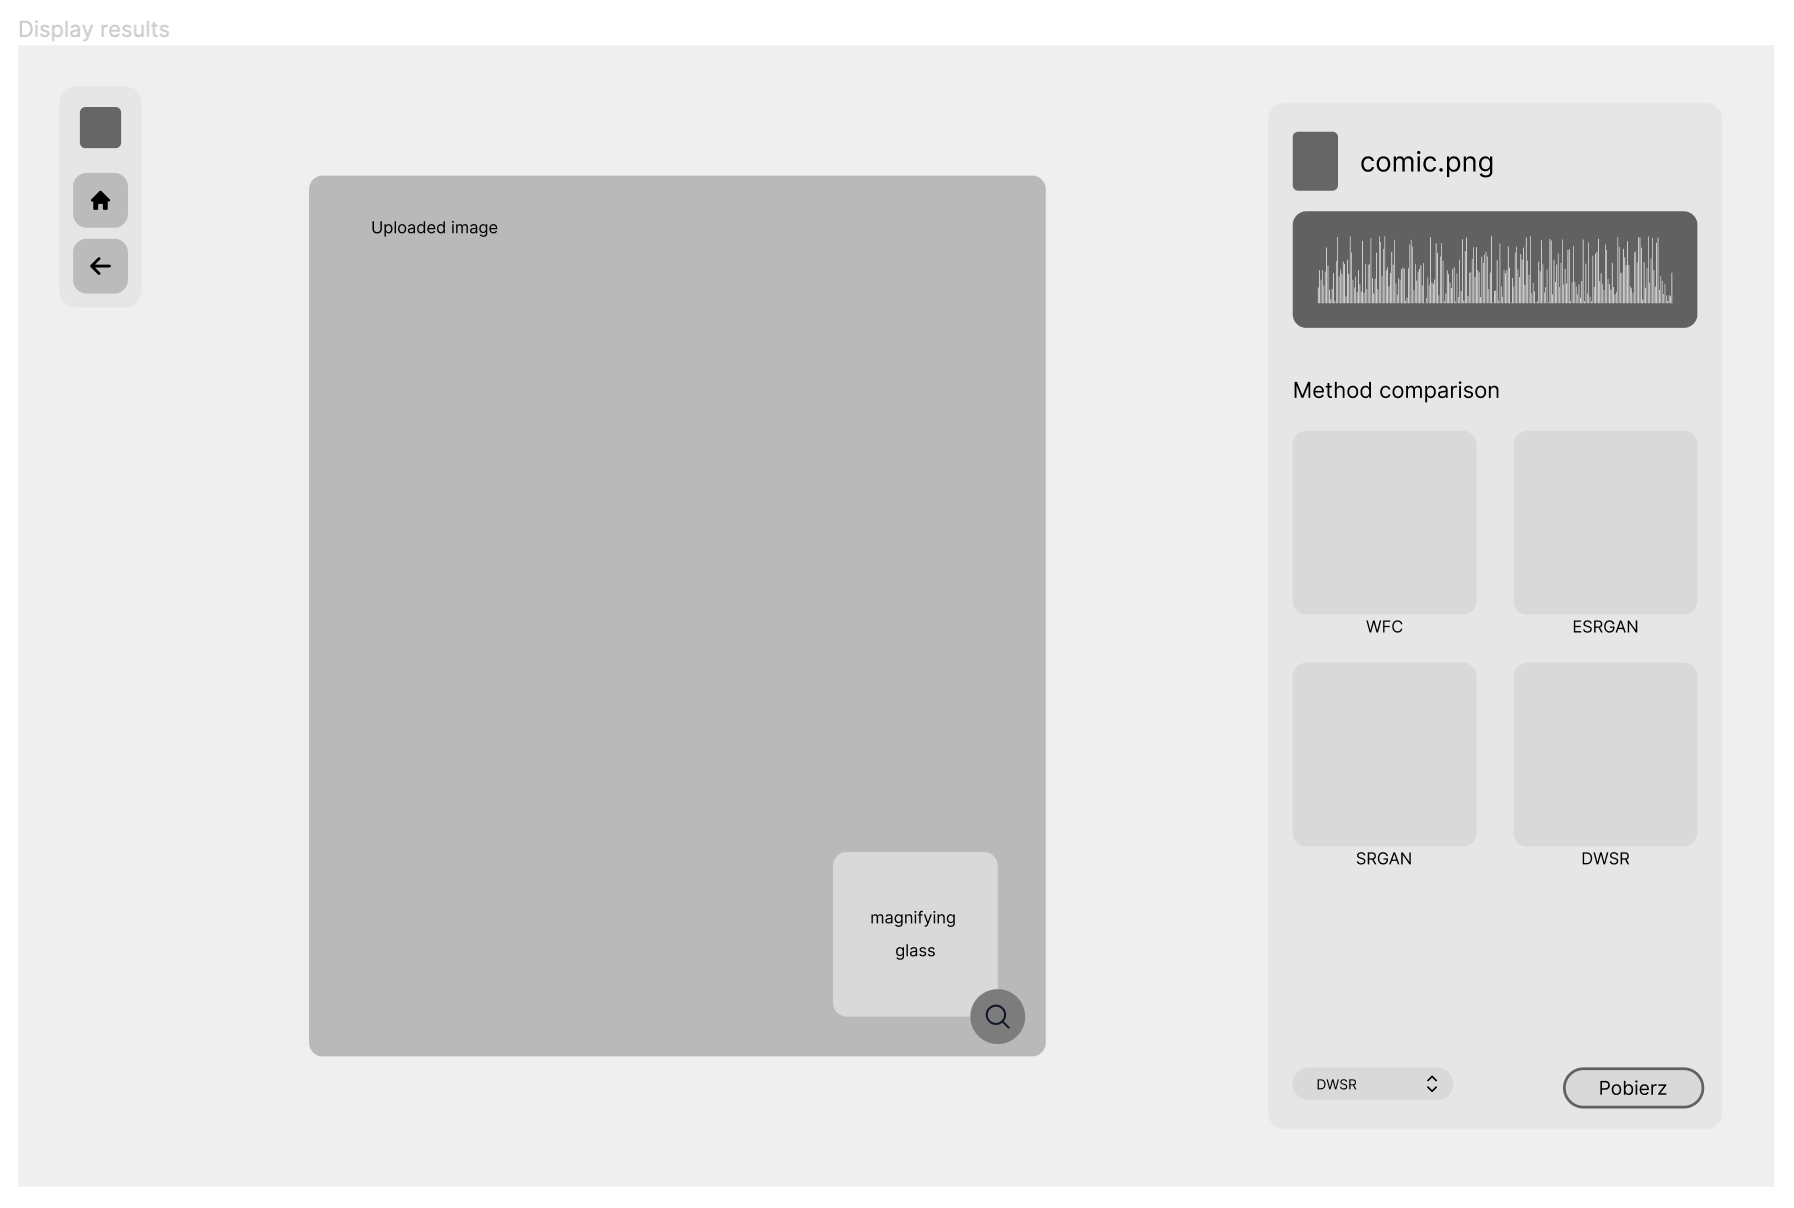
\includegraphics[width=0.8\linewidth]{Rozdziały/06.Aplikacja/Obrazy/UX display.png}  
    \caption{Pierwsza wersja UX aplikacji (ekran prezentacji wyników)}
    \label{fig:image84}
\end{figure}

Pierwotny rozkład elementów na stronie różni się od tego jak to wygląda teraz. Wraz z rozwojem aplikacji zmieniałem układ elementów, usprawniałem interakcję z użytkownikiem i poprawiałem rozkład elementów na ekranach aplikacji.

Kolejnym etapem pracy był projekt graficzny aplikacji. Zdecydowałem, że aplikacja będzie w ciemnym motywie, gdyż taki styl pomaga nam skupić się na tym co jest na ekranie, zwłaszcza w kontekście edycji zdjęć. Zależało mi na tym, żeby aplikacja nie była jednowymiarowa i żeby wyglądała nowocześnie. Początkowo eksperymentowałem z grafikami wektorowymi w tle [Rys \ref{fig:image85}], lecz ten wygląd nie przekonywał mnie. Eksperymentując z wyglądem pomyślałem, że w nawiązaniu do szumu na zdjęciach analogowych, tło aplikacji może mieć szum, zaś jako że mamy do czynienia z nowoczesnym narzędziem to kursor i elementy UI będą przejrzyste i czyste. W ten sposób aplikacja zyskuje na głębi i tak wygląda aktualna wersja, którą postanowiłem zaimplementować [Rys \ref{fig:image80}].

\begin{figure}[H]
    \centering
    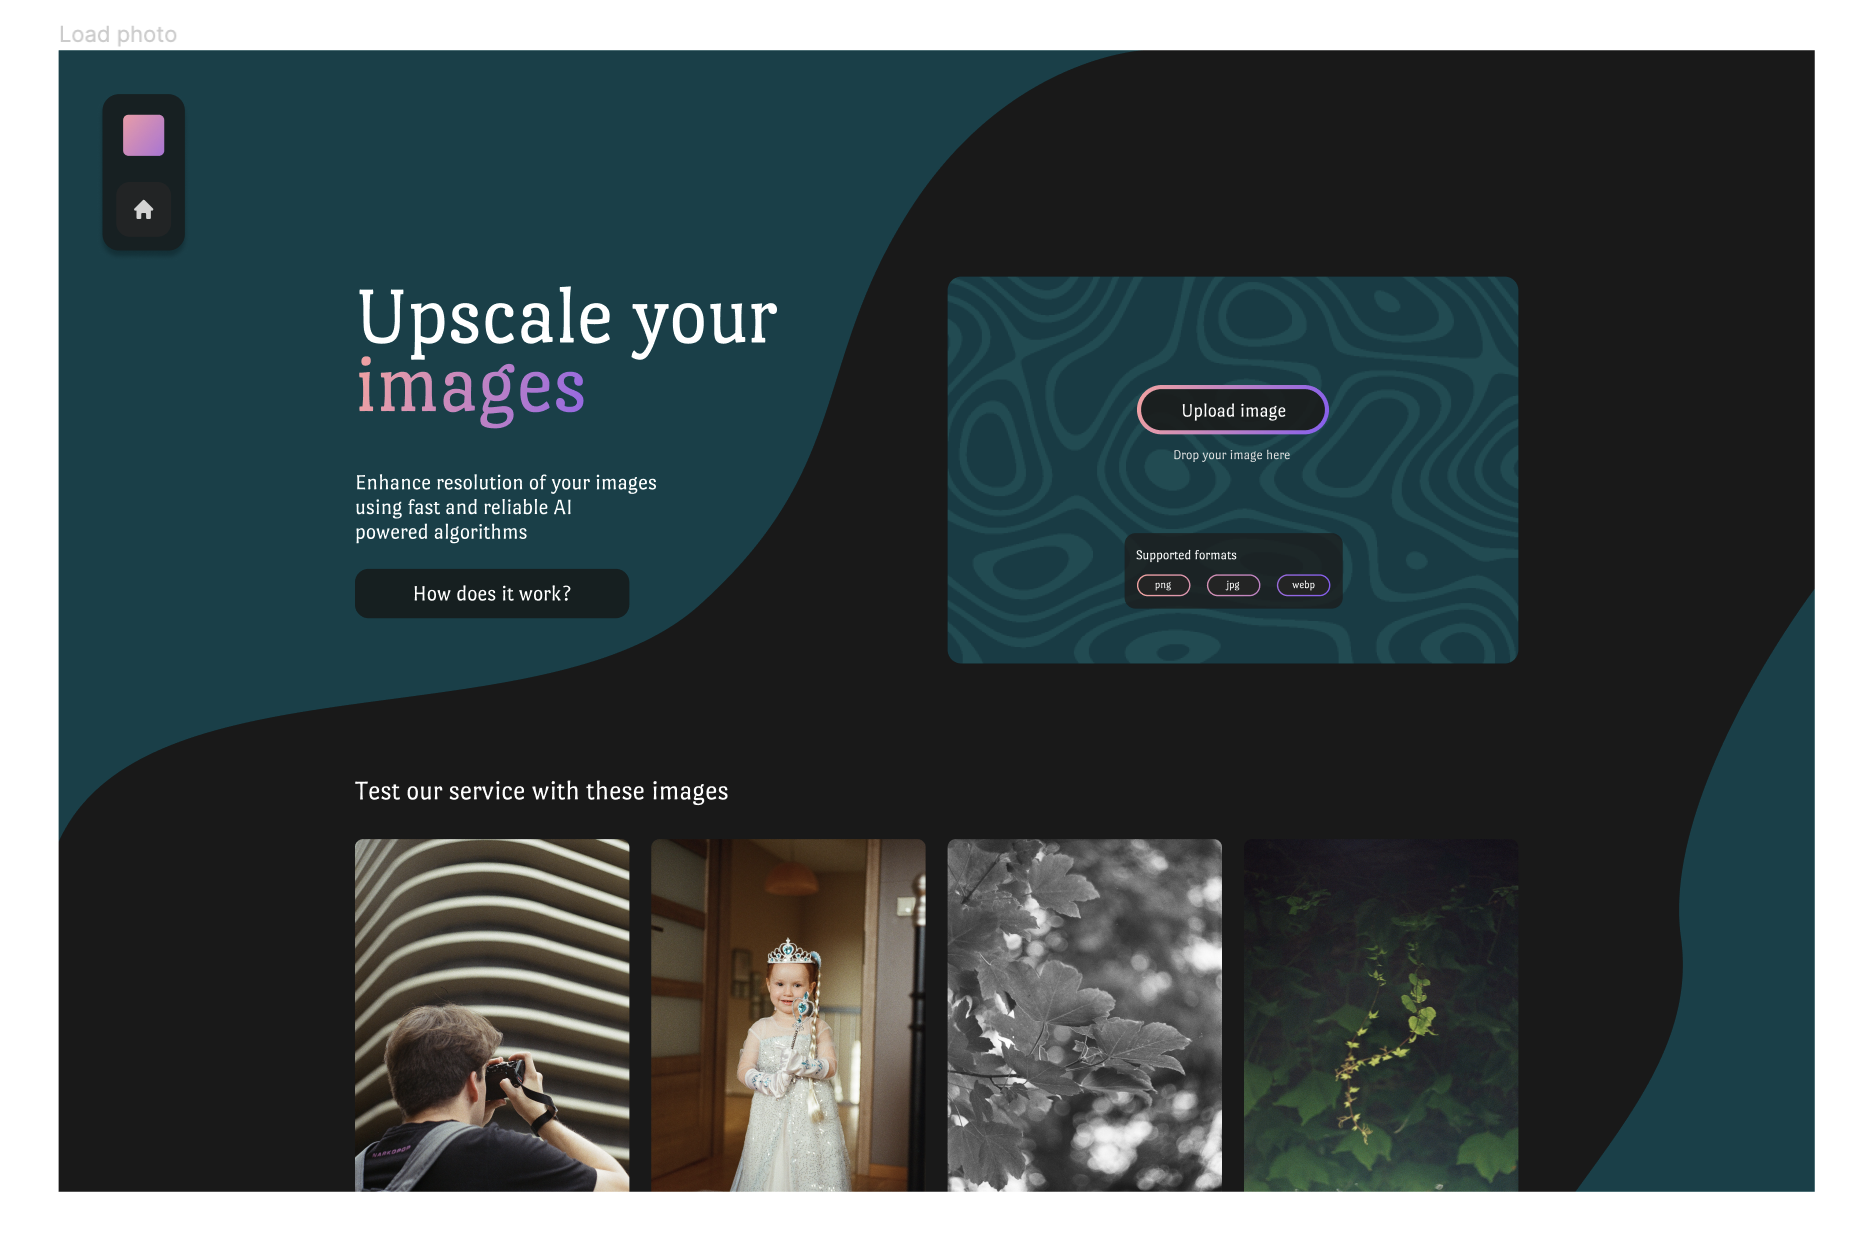
\includegraphics[width=0.8\linewidth]{Rozdziały/06.Aplikacja/Obrazy/UI 1.png}  
    \caption{Pierwsza wersja UI strony głównej}
    \label{fig:image85}
\end{figure}

Podobnie wyglądał proces projektowania ekranu prezentacji wyników [Rys \ref{fig:image86}]. Zdecydowałem, żeby na ekranie prezentacji wyników były tylko istotne elementy interfejsu, żeby użytkownik nie pogubił się w nadmiarze informacji. Zależało mi na tym, żeby użytkownik mógł łatwo porównać wyniki różnych algorytmów, dlatego zdecydowałem się na układ kafelków, które można wybrać i porównać z sobą. Dodatkowo w tych kafelkach uznałem, że świetnie sprawdzi się widok z bliska, który pozwoli na dokładne przyjrzenie się szczegółom obrazu, tak powstała lupka, która podąża za kursorem gdy wskaźnik znajduje się nad obrazem. 


\begin{figure}[H]
    \centering
    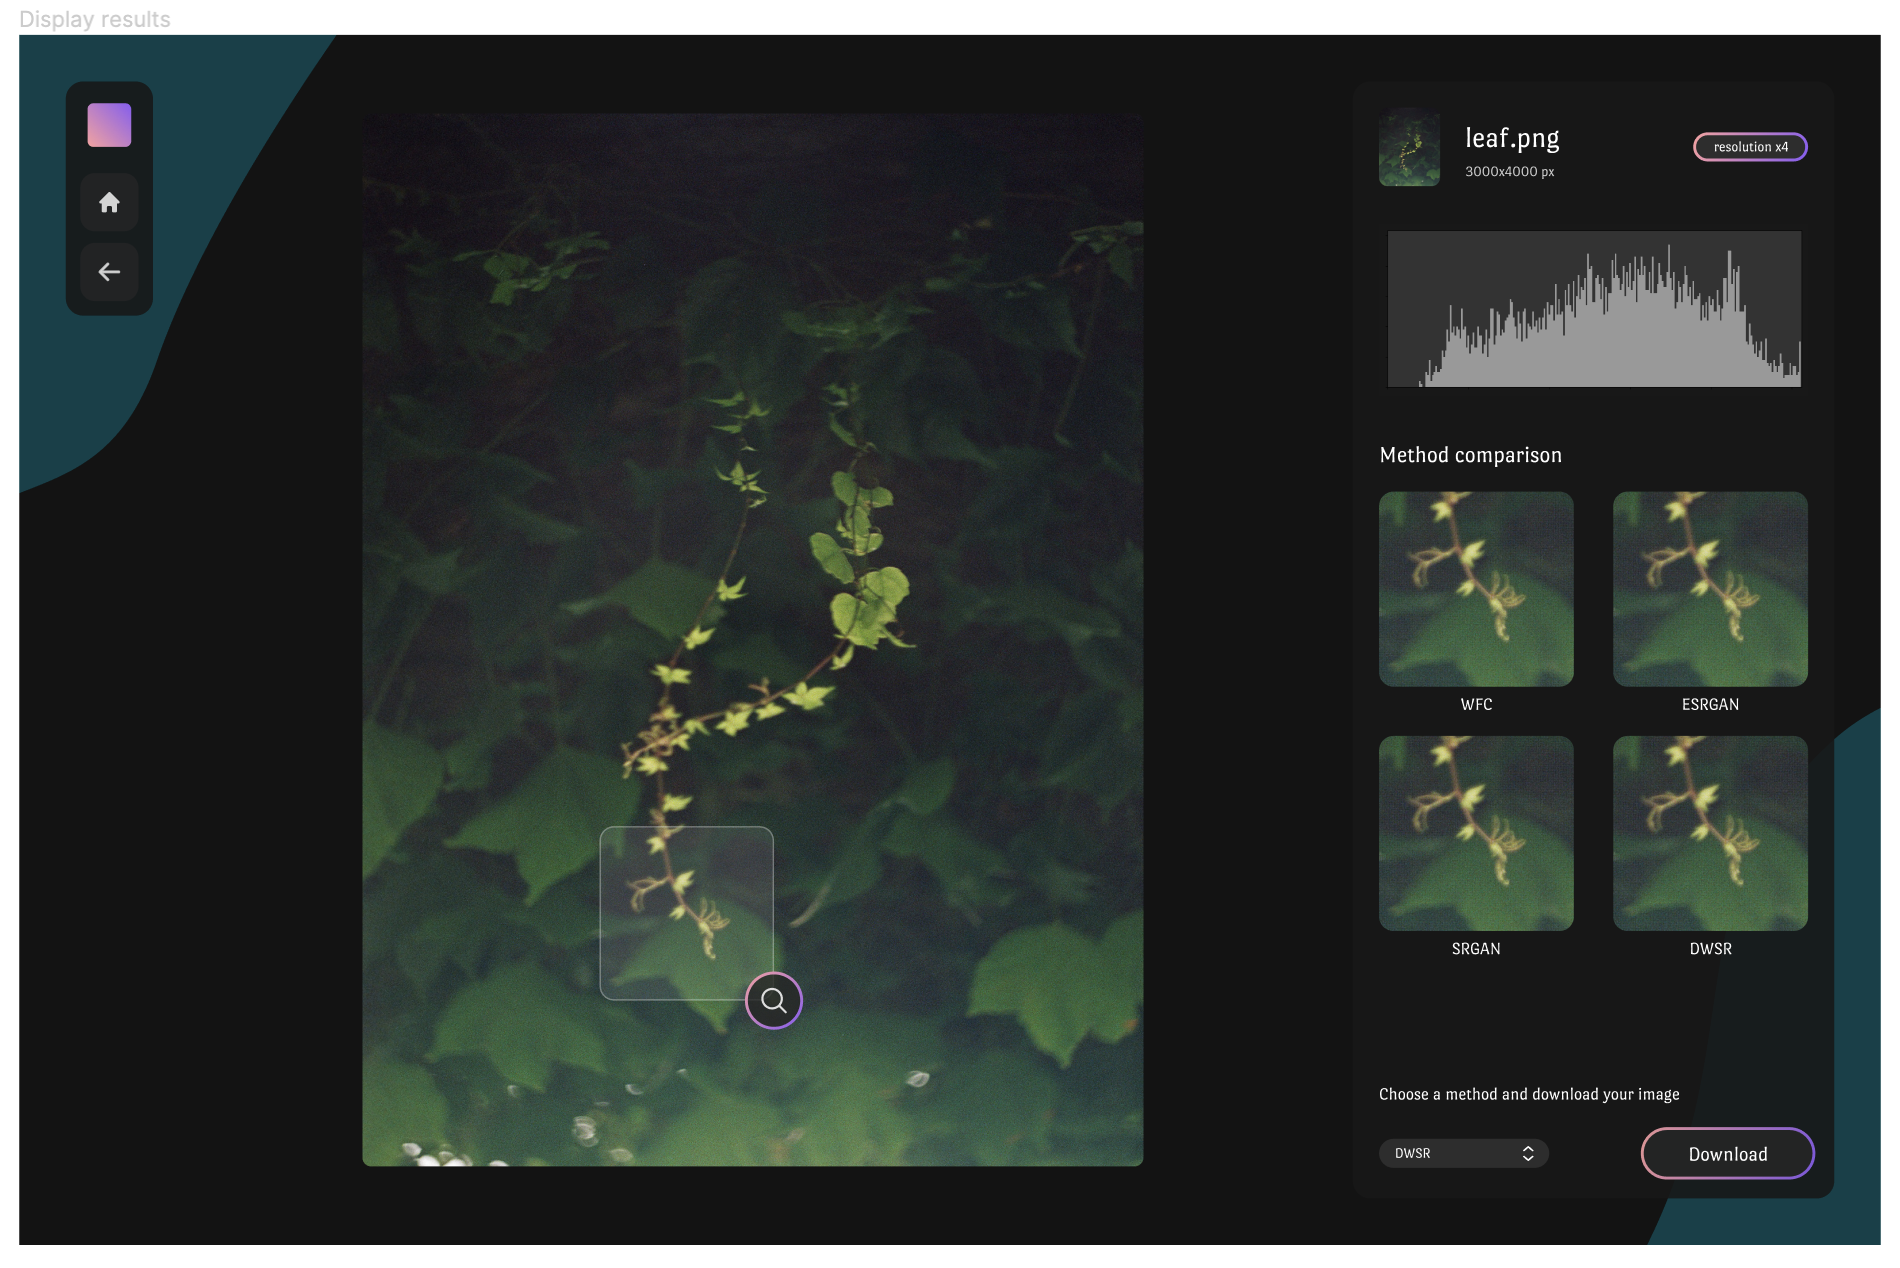
\includegraphics[width=0.8\linewidth]{Rozdziały/06.Aplikacja/Obrazy/UI 1 dsiplay .png}  
    \caption{Pierwsza wersja UI ekranu wyświetlania wyników}
    \label{fig:image86}
\end{figure}

W kolejnej wersji widoku prezentacji wyników postanowiłem zmienić wygląd tła. Zainspirowany aplikacjami typu \textbf{Apple Music} czy \textbf{Spotify} zdecydowałem się na zmianę tła na gradient z kolorów występujących na obrazie. W ten sposób aplikacja zyskuje na głębi i wygląda bardziej nowocześnie [Rys \ref{fig:image81}]. W tym miejscu projekt aplikacji uznałem za gotowy do implementacji, gdzieś trzeba się zatrzymać, żeby sprawdzić jak działają mechanizmy w praktyce. O planach rozbudowy aplikacji traktuję rozdział \ref{sec:plans}.



\section{Wybór narzędzi i technologii}

Kolejnym krokiem w tworzeniu aplikacji jest decyzja odnośnie używanych technologii i narzędzi. W tym rozdziale opiszę jakie technologie i narzędzia wybrałem do stworzenia aplikacji webowej.


\subsection*{Vue.js: Frontend}

Do implementacji Frontendu zdecydowałem się na użycie frameworku \textbf{Vue.js}


\textbf{Vue.js} to progresywny framework JavaScript służący do budowania interfejsów użytkownika. Został stworzony przez Evana You i jest utrzymywany przez niezależnych współtwórców z całego świata. Jego elastyczność pozwala na łatwą integrację z innymi bibliotekami lub istniejącymi projektami, a także jest świetny do tworzenia zaawansowanych aplikacji jednostronicowych (SPA - Single Page Applications). Swietnie nada się do tego projektu, gdyż jest to niewielka aplikacja, która będzie korzystać z wielu bibliotek i narzędzi.


\subsubsection*{Architektura i Komponenty}

Architektura Vue opiera się na systemie komponentów. Komponenty w Vue są blokami wielokrotnego użytku z własnym stanem, metodami i szablonami. Dzięki temu łatwo jest tworzyć interfejsy składające się z mniejszych, niezależnych części, co znacznie ułatwia zarządzanie, utrzymanie i czytelność kodu.

\subsubsection*{Reaktywność i Dwukierunkowe Wiązanie Danych}

Jedną z kluczowych cech Vue.js jest jego reaktywny system, który zapewnia automatyczną aktualizację interfejsu użytkownika w odpowiedzi na zmiany stanu aplikacji. Framework ten używa systemu dwukierunkowego wiązania danych (two-way data binding), co oznacza, że zmiany w modelu danych od razu są odzwierciedlane w widoku i na odwrót.

\subsubsection*{Deklaratywne Renderowanie}

Vue.js wykorzystuje deklaratywne renderowanie. Oznacza to, że developer określa, jakie dane powinny być wyświetlane, a framework zajmuje się ich aktualizacją w widoku. To sprawia, że kod jest bardziej zrozumiały i łatwiejszy w utrzymaniu.

\subsubsection*{Virtual DOM}

Vue korzysta z koncepcji Virtual DOM, co pozwala na efektywną aktualizację widoku bez konieczności odświeżania całej strony. Jest to znacznie szybsze niż tradycyjne manipulowanie DOM, ponieważ zmiany są najpierw aplikowane do Virtual DOM, a następnie, w optymalny sposób, przekazywane do rzeczywistego DOM.

\subsubsection*{Ekosystem i Społeczność}

Vue ma rozbudowany ekosystem, w skład którego wchodzą takie narzędzia jak Vue Router (do zarządzania routingiem w SPA) i Vuex (do zarządzania stanem aplikacji). Dodatkowo, wsparcie społeczności i dostępność zasobów edukacyjnych, takich jak dokumentacja, tutoriale i fora dyskusyjne, sprawiają, że nauka i praca z Vue.js jest dostępna i przyjemna.




\subsection*{Django: Backend}



Django to wysokopoziomowy framework webowy napisany w Pythonie, który umożliwia szybkie tworzenie bezpiecznych i utrzymywalnych stron internetowych. Został zaprojektowany z myślą o uproszczeniu zadań związanych z tworzeniem aplikacji internetowych, dzięki czemu deweloperzy mogą skupić się na pisaniu aplikacji bez konieczności ponownego wynajdywania koła.

\subsubsection*{Architektura Wzorca Projektowego MTV}

Django wykorzystuje wzorzec projektowy "Model-Template-View" (MTV), który jest podobny do popularnego wzorca MVC. W tym podejściu:
\begin{itemize}
    \item \textbf{Model} odpowiada za strukturę danych oraz ich walidację.
    \item \textbf{Template} zajmuje się prezentacją danych, czyli warstwą frontendową.
    \item \textbf{View} odpowiada za logikę aplikacji, odbierając żądania od użytkownika i zwracając odpowiednie odpowiedzi.
\end{itemize}

\subsubsection*{ORM (Object-Relational Mapping)}

Django zawiera wbudowany ORM, który pozwala na interakcję z bazami danych za pomocą kodu Python, zamiast pisać surowe zapytania SQL. ORM przekształca tabele bazy danych w klasy Pythona, co ułatwia manipulowanie danymi i sprawia, że kod jest bardziej czytelny i bezpieczny.

\subsubsection*{Bogata Funkcjonalność "Out-of-the-Box"}

Django oferuje wiele wbudowanych funkcji "out-of-the-box", takich jak system autentykacji użytkowników, mapowanie URL na widoki, mechanizm szablonów, system administrowania itd. Dzięki temu można szybko rozpocząć pracę nad projektem, mając już na starcie zestaw potrzebnych narzędzi.

\subsubsection*{Bezpieczeństwo}

Bezpieczeństwo jest jedną z głównych zalet Django. Framework ten automatycznie chroni aplikacje przed wieloma powszechnymi zagrożeniami, takimi jak SQL Injection, Cross-site Scripting (XSS), Cross-site Request Forgery (CSRF) i Clickjacking, dzięki czemu deweloperzy mogą skupić się na budowaniu aplikacji, nie martwiąc się o podstawowe kwestie bezpieczeństwa.

\subsubsection*{Skalowalność i Wersjonowanie}

Django jest skalowalny i może obsługiwać zarówno małe, jak i duże projekty. Ponadto, framework ten wspiera koncept wersjonowania API, co jest kluczowe przy rozwijaniu i utrzymywaniu dużych aplikacji.

\subsubsection*{Wsparcie Społeczności i Dokumentacji}

Podobnie jak w przypadku Vue.js, Django ma silną i aktywną społeczność. Dzięki temu deweloperzy mają dostęp do bogatej dokumentacji, licznych zasobów edukacyjnych i gotowych rozwiązań, co ułatwia naukę i rozwiązywanie problemów.







\section{Implementacja aplikacji}



Opis technicznego procesu integracji wybranych algorytmów z aplikacją, wraz z napotkanymi wyzwaniami.

K-means algorytm do detekcji kolorów wystepujacych na obrazie.



\section{Integracja algorytmów DWSR i ESRGAN}




\section{Testowanie aplikacji}




\section{Wdrożenie i utrzymanie aplikacji}

Omówienie procesu wdrożenia gotowej aplikacji oraz planów dotyczących jej przyszłego utrzymania i aktualizacji.



\section{Plany na przyszłość} \label{sec:plans}

Opis błędów, rzeczy do poprawy w aplikacji. Omówienie jakie są plany rozbudowy aplikacji.